\documentclass[10pt,a4paper]{scrartcl}
\PassOptionsToPackage{table}{xcolor}
\usepackage[utf8]{inputenc}
\usepackage[T1]{fontenc}
\usepackage[ngerman]{babel}
\usepackage{microtype, multicol, marginnote, bera, parskip}
\usepackage{listings, amsmath, amssymb, graphicx, tikz, epic}
\usepackage{stmaryrd} %for lightning arrow
\usepackage{pstricks, pst-node, pst-tree, pdflscape}
\usepackage[babel=true]{csquotes}
\usepackage{placeins}
\usepackage[labelformat=empty]{caption}
\tolerance=2000
\setcounter{secnumdepth}{0}
\usepackage[inner=2cm,outer=2cm,top=1.5cm,bottom=1.5cm,includeheadfoot]{geometry}
\usepackage{multirow}
\newcommand{\subExercise}[1]{\vspace{0.5em} \noindent{\bf #1)}}
\DeclareMathOperator{\op}{op}

\author{Michael Mardaus \and Andrey Tyukin}
\title{
\includegraphics[scale=0.2]{../logo_schriftzug}\\
Technische Informatik: Abgabe 7}

\begin{document}

\maketitle

\section*{Exercise 7.1 (Flipflop logical simulation)}
Let FF1 be a $0\rightarrow 1$ flank controlled D-flipflop and FF2 a $1\rightarrow0$ flank controlled one.\\
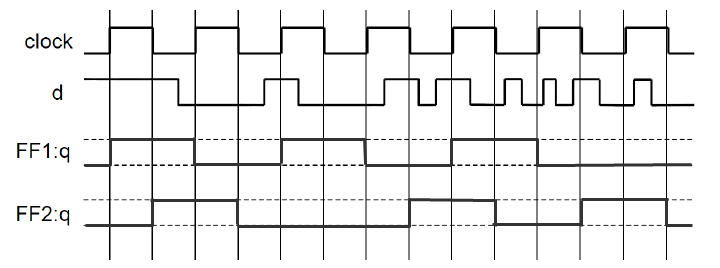
\includegraphics[width=\textwidth]{images/flipflop-sim.png} 

\FloatBarrier
\section*{Exercise 7.2 (Flipflops)}


\FloatBarrier
\section*{Exercise 7.3 (Gum machine)}

We contructed an automaton with 4 states, as we do not differentiate between 15 cents and 20 cents (and even more cents). (That way we have smaller tables.) 
\begin{itemize}
\item state 00 means 0 cents balance
\item state 01 means 10 cents balance
\item state 10 means 5 cents balance
\item state 11 means \glqq enough cents\grqq \ balance ( $\geq 15$ )
\end{itemize}

We have one input bit $w$, which is 0 if a 5 cent coin is insered and 1 if a 10 cent coin is inserted. That gives us the following state/output table:


\begin{tabular}{|c||c|c||c|c|}
  \hline
 State   & \multicolumn{2}{c||}{Next state} & \multicolumn{2}{c|}{Output} \\
         & $w=0$        & $w=1$            & $w=0$       & $w=1$ \\
$y_1y_0$ & $Y_1Y_0$     & $Y_1Y_0$         & $z$         & $z$   \\ \hline\hline
00       & 10           & 01               & 0           & 0     \\ \hline  
01       & 11           & 11               & 0           & 0     \\ \hline
10       & 01           & 11               & 0           & 0     \\ \hline
11       & 11           & 11               & 1           & 1     \\ \hline
\end{tabular}

We extract the K-maps for $Y_0$ and $Y_1$ and $z$ and get

\begin{tabular}{|c||c|c|c|c|}
  \hline
\textcolor{red}{$Y_0$}    & \multicolumn{4}{c|}{$y_1y_0$} \\
$w$    & 00 & 01  & 11  & 10\\ \hline\hline
  0    &    & 1   & 1   & 1 \\ \hline
  1    & 1  & 1   & 1   & 1 \\ 
  \hline
\end{tabular}
\hspace{1cm}
\begin{tabular}{|c||c|c|c|c|}
  \hline
\textcolor{red}{$Y_1$}     & \multicolumn{4}{c|}{$y_1y_0$} \\
$w$    & 00 & 01  & 11  & 10\\ \hline\hline
  0    & 1  & 1   & 1   &   \\ \hline
  1    &    & 1   & 1   & 1 \\ 
  \hline
\end{tabular}
\hspace{1cm}
\begin{tabular}{|c||c|c|c|c|}
  \hline
\textcolor{red}{$z$}   & \multicolumn{4}{c|}{$y_1y_0$} \\
$w$    & 00 & 01  & 11  & 10\\ \hline\hline
  0    &    &     & 1   &   \\ \hline
  1    &    &     & 1   &   \\ 
  \hline
\end{tabular}

$Y_0=w+y_0+y_1\qquad\qquad\qquad\qquad\quad Y_1=\bar{w}\bar{y_1} + y_0 + wy_1\qquad\qquad\qquad\quad z=y_1y_2$

and that leads us to this circuit:\\
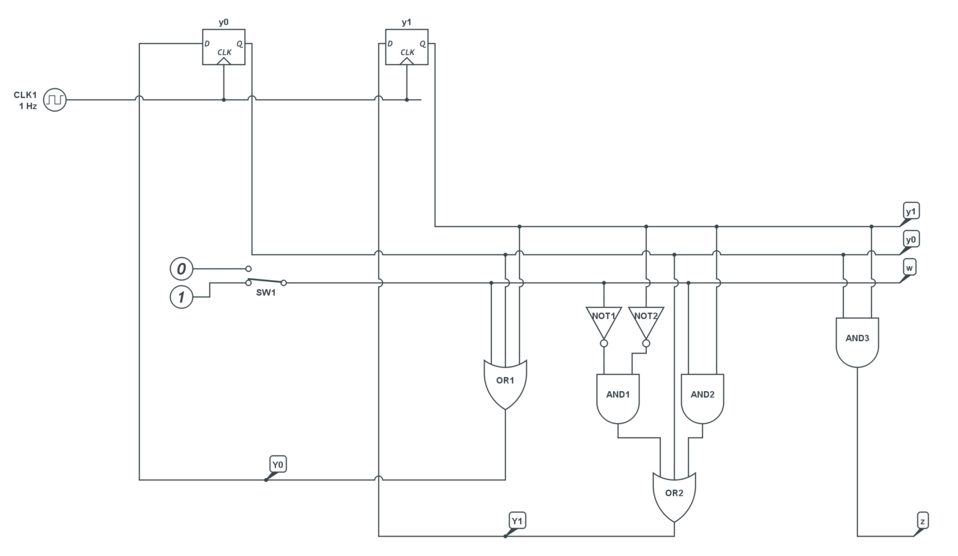
\includegraphics[width=\textwidth]{images/automat.png} 


\FloatBarrier
\section*{Exercise 7.4 (Neumann-Adder)}

\end{document}
